\chapter{Results}
\label{sec:results}

\section{Findings from the Simulations}
- Wie in Vorversuchen schon bemerkt: QE-Schema produziert numerische Fehler, die sich darin zeigen, dass Preise mehrfach in der Simulation vorkommen. Bei korrekter Simulation ist der häufigste Preis im ersten Pfad im einstelligen Bereich, bei Fehlern im Hunderter- oder Tausenderbereich.
- Abbildung \ref{fig:max_number_of_same_prices_distribution} zeigt die Verteilung, man sieht einen Peak bei 1, was darauf hindeutet, dass die meisten Simulationen korrekt sind. Man sieht aber auch, dass es einige Simulationen gibt, wo der selbe Preis bis zu 250000 mal vorkommt, hier kam es zu numerischen Fehlern. Bei diesen Simulationen stellt man fest, dass, wenn es das erste Mal zu numerischen Fehlern kommt, der Rest der Zeitreihe den selben Preis hat. Bei Simulationen mit 250000 gleichen Preises kam es also sehr früh in der Zeitreihe zu einem numerischen Fehler.

\begin{figure}
    \centering
    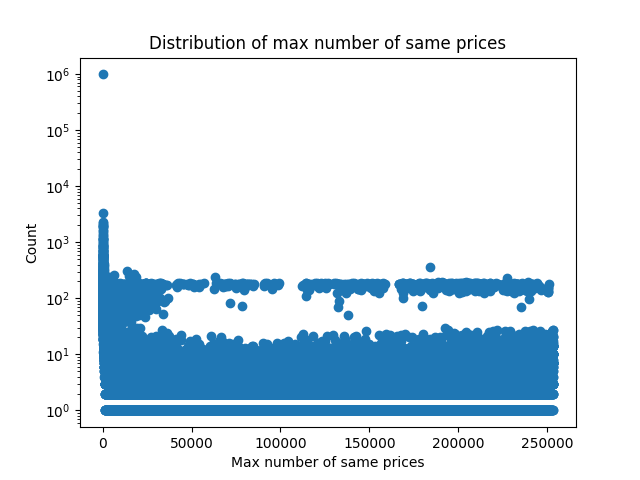
\includegraphics[width=0.8\textwidth]{img/max_number_of_same_prices_distribution.png}
    \caption{Distribution of the maximum number of the same prices in the first path of the simulation}
    \label{fig:max_number_of_same_prices_distribution}
\end{figure}

- Für die weitere Untersuchung sollen solche Simulationen ausgeschlossen werden, da sie nicht korrekt sind. Da es durchaus möglich ist, dass es auch bei korrekter Simulation zu gleichen Preisen kommt, wird ein Schwellwert gesucht, sodass möglichst viele korrekte Simulationen in der Untersuchung bleiben. Abbildung \ref{fig:max_number_of_same_prices_cumulative_percentage} zeigt für verschiedene Schwellwerte (die maximale Anzahl an gleichen Preisen) den kumulativen Anteil der Simulationen, die diesen Schwellwert nicht überschreiten. Wählt man den Schwellwert 1, also nur Simulationen, bei denen nie ein Preis mehrfach vorkommt, verbleiben bleiben 68.40\% der Simulation. Je höher man den Schwellwert setzt, desto weniger Simulationen fallen weg, aber unter Umständen verbleiben auch Simulationen, die numerische Fehler enthalten. Das betrifft aber nur sehr wenige Simulationen, der Anteil an inkludierten Simulationen steigt fast gar nicht. Für die späteren Untersuchungen werden also alle Simulationen entfernt, bei denen der selbe Preis mehr als einmal vorkommt.

\begin{figure}
    \centering
    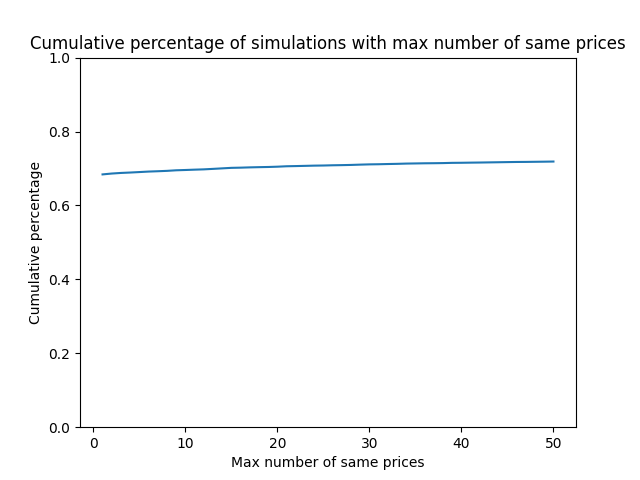
\includegraphics[width=0.8\textwidth]{img/max_number_of_same_prices_cumulative_percentage.png}
    \caption{Cumulative percentage of simulations that do not exceed the maximum number of same prices}
    \label{fig:max_number_of_same_prices_cumulative_percentage}
\end{figure}

\begin{figure}
    \centering
    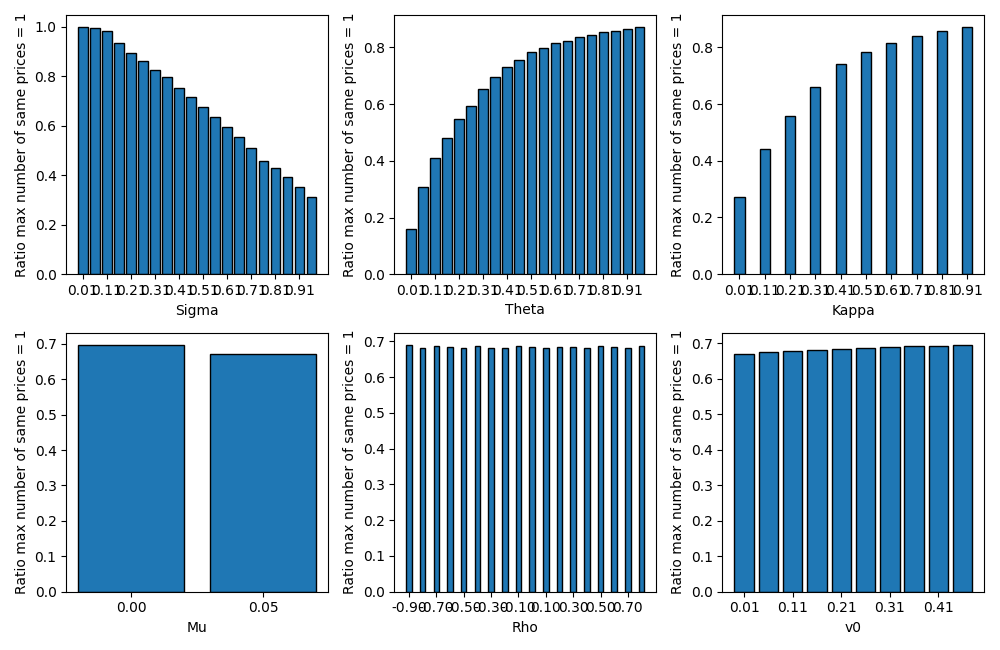
\includegraphics[width=0.8\textwidth]{img/max_number_of_same_prices_ratio_parameters.png}
    \caption{Ratio of simulations that do not exceed the maximum number of same prices in relation to the parameters of the Heston model}
    \label{fig:max_number_of_same_prices_ratio_parameters}
\end{figure}

\begin{figure}
    \centering
    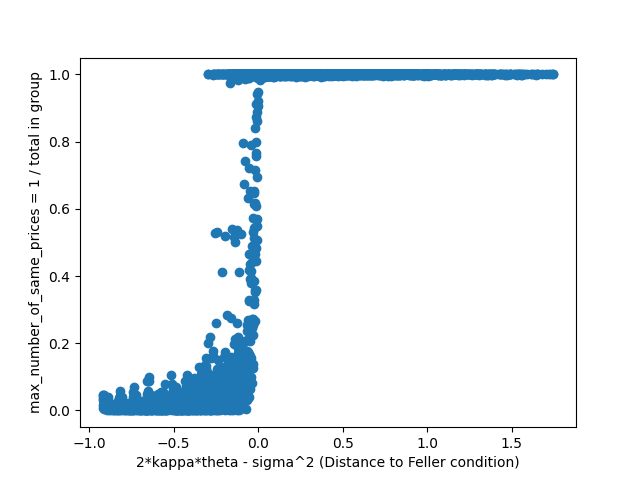
\includegraphics[width=0.8\textwidth]{img/max_number_of_same_prices_ratio_feller_diff.png}
    \caption{Ratio of simulations that do not exceed the maximum number of same prices in relation to the value $D$}
    \label{fig:max_number_of_same_prices_ratio_D}
\end{figure}

- Untersuchung, woher diese Fehler kommen: Dazu bestimmen des Anteils der Simulationen, die korrekt in Abhängigkeit eines jeden einzelnen Parameters des Heston-Modells (siehe Abbildung \ref{fig:max_number_of_same_prices_ratio_parameters}). Man erkennt, dass mit zunehmendem $\sigma$ die Fehler zunehmen, während mit zunehmendem $\theta$ und $\kappa$ die Fehler abnehmen. Die Parameter $\mu$, $\rho$ und $v_0$ haben keinen Einfluss auf die Fehlerhäufigkeit. Das legt nahe, dass die Fehler mit der Feller condition zusammenhängen. Deshalb untersuche ich nun die Fehlerhäufigkeit und den Wert $D = 2\kappa\theta - \sigma^2$. Ist dieser Wert positiv, so ist die Feller condition erfüllt, je negativer er ist, desto weniger erfüllt ist die Feller condition. Abbildung \ref{fig:max_number_of_same_prices_ratio_D} zeigt, dass, sobald die Feller condition nicht mehr erfüllt ist, die Fehlerhäufigkeit stark zunimmt. Wenn die Feller condition erfüllt ist, so sind 99.90\% der Simulationen korrekt, ist die Feller condition nicht erfüllt, so sind es nur 25.48\%. Insgesamt erfüllen 57.80\% der Simulationen die Feller condition.
- Im Folgenden wird untersucht, in welchen Szenrien welche Expansionsmethoden die theoretische Verteilung am besten approximieren. Für gegebene Level an Skewness und Kurtosis wird analysiert, wie gut sich die Gram-Charlier-Expansion eignet. Nutzung der Gram-Charlier-Expansion, da dies die einfachste Methode ist. In einem zweiten Teil wird dann untersucht, inwiefern es Unterschiede in den Expansionsmethoden gibt, wie sie die Verteilung allgemein approximieren und wie sie die Tails approximieren können. Zudem wird dabei auch auf die Feller condition eingegangen, wie diese die Ergebnisse beeinflusst.
- In der Auswertung fokussieren wir uns nur auf Simulationen mit $\mu=0$, da bei $\mu=0.05$ sehr viele Simulationen fehlerhaft sind. Zudem betrachten wir nur Simulationen, in denen die Feller condition erfüllt ist, da bei nicht erfüllter Feller condition insbesondere die Werte für die theoretische Skewness und theoretische Kurtosis extreme Werte annehmen (siehe Abbildung \ref{fig:kde_theoretical_skewness_kurtosis_feller_false}).

\begin{figure}
    \centering
    \begin{subfigure}[b]{0.4\textwidth}
        \centering
        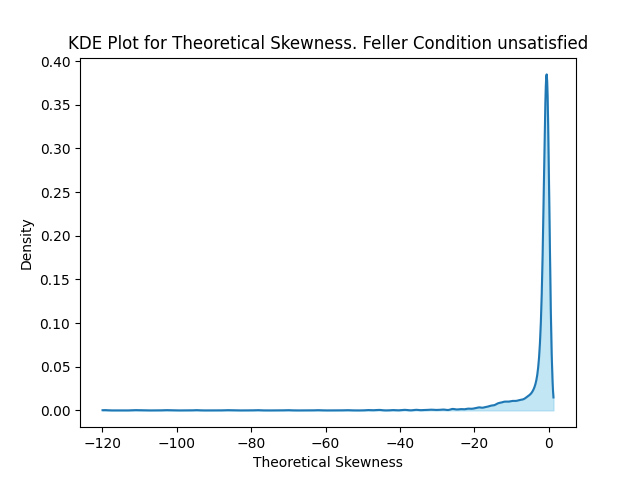
\includegraphics[width=\textwidth]{img/kde_theoretical_skewness_feller_false.png}
        \caption{Theretical Skewness}
    \end{subfigure}
    \hfill
    \begin{subfigure}[b]{0.4\textwidth}
        \centering
        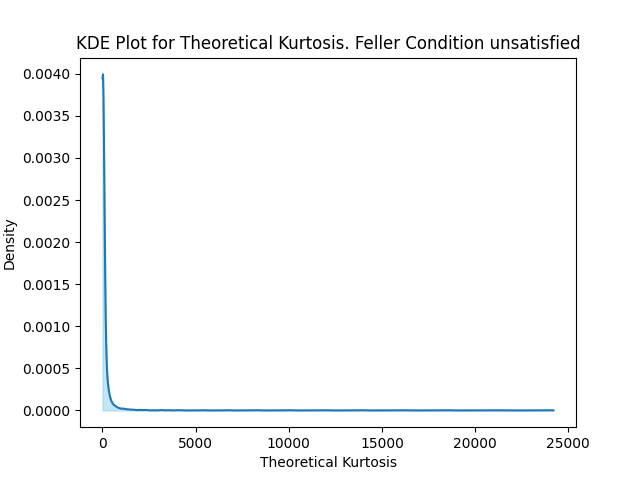
\includegraphics[width=\textwidth]{img/kde_theoretical_kurtosis_feller_false.png}
        \caption{Theoretical Kurtosis}
    \end{subfigure}
    \caption{Kernel density estimation of the theoretical skewness and kurtosis for simulations where the Feller condition is not fulfilled}
    \label{fig:kde_theoretical_skewness_kurtosis_feller_false}
\end{figure}

\section{Investigating the Results for the Gram-Charlier-Expansion with respect to Skewness und Kurtosis}

\begin{figure}
    \centering
    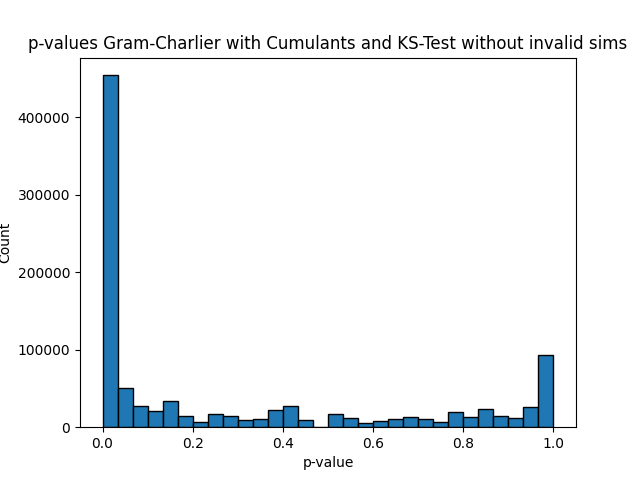
\includegraphics[width=0.8\textwidth]{img/GC_cum_KS_p_value_histogram.png}
    \caption{Distribution of p values of the Kolmogorov-Smirnov-Test for the Gram-Charlier Expansion with Cumulants vs the theoretical density without invalid simulations}
    \label{fig:GC_cum_KS_p_value_histogram}
\end{figure}

- In Abbildung \ref{fig:GC_cum_KS_p_value_histogram} sieht man die Verteilung der p values des Kolmogorov-Smirnov-Tests für die Gram-Charlier Expansion mit Kumulanten im Vergleich zur theoretischen Dichte. Dabei wurden alle Simulationen entfernt, bei denen der selbe Preis mehr als einmal vorkommt. Ein p Wert von über 5\% bedeutet, dass es keine signifikanten Unterschiede zwischen den beiden Verteilungen gibt, die Gram-Charlier Expansion auf Basis von Kumulanten approximiert die theoretische Dichte also gut genug. Man sieht, dass dies für einige Parameterkombinationen nicht der Fall ist; insgesamt für 52.48\% der Simulationen. Für restliche Expansionsmethoden siehe Tabelle \ref{tab:KS_p_value_percentage}.

\begin{table}[h]
    \centering
    \begin{tabular}{l|c|c|c|c|c|c}
        & \textbf{Gram-Charlier} & \textbf{GC+} & \textbf{Edgeworth} & \textbf{EW+} & \textbf{Cornish-Fisher} & \textbf{Saddlepoint} \\
        \hline
        \textbf{Cumulants} & 52.48\% & 47.63\% & 52.14\% & 47.64\% & 35.85\% & 45.36\% \\
        \textbf{Moments} & 37.35\% & 21.24\% & 36.02\% & 23.27\% & 44.90\% & 40.92\%
    \end{tabular}
    \caption{Percentage of simulations where the p-value of the Kolmogorov-Smirnov-Test against the theoretical density is above 5\%. Invalid simulations are excluded. GC+ and EW+ stand for the Gram-Charlier Expansion with positivity constraint and the Edgeworth Expansion with positivity constraint, respectively.}
    \label{tab:KS_p_value_percentage}
\end{table}

- Weiterhin erkennt man in Tabelle \ref{tab:KS_p_value_percentage}, dass die Expansionsmethoden besser mit der Methode der Kumulanten als mit der Methode der Momente abschneiden. Die Cornish-Fisher Expansion und die Saddlepoint Approximation, die in Kapitel \ref{sec:literature} kurz angerissen worden sind, scheiden am schlechtesten ab und werden deshalb in den weiteren Untersuchungen nicht weiter betrachtet, genau so wie die Expansionsmethoden auf Basis von Momenten. Der Grund, warum die Methode der Kumulanten besser abschneidet, ist, dass diese die theoretische Skewness und Kurtosis des Heston Modells besser einfangen als die Methode der Momente, wie man in Abbildung \ref{fig:theoretical_vs_real_skewness_kurtosis} sieht. Die Skewness und Kurtosis von Neuberger \& Payne (2021) sind direkt aus den Momenten berechnet, Neuberger and Payne haben es auch so in ihrem Paper beschrieben. %TODO: darauf achten, dass "einfangen" mit "capture" übersetzt wird

\begin{figure}
    \centering
    \begin{subfigure}[b]{0.4\textwidth}
        \centering
        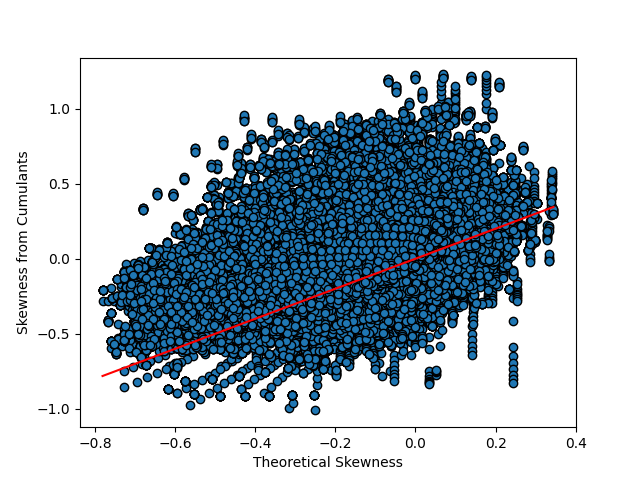
\includegraphics[width=\textwidth]{img/theoretical_skewness_vs_skewness_from_cumulants_feller_condition_true.png}
        \caption{Theretical Skewness vs Skewness from Cumulants}
    \end{subfigure}
    \hfill
    \begin{subfigure}[b]{0.4\textwidth}
        \centering
        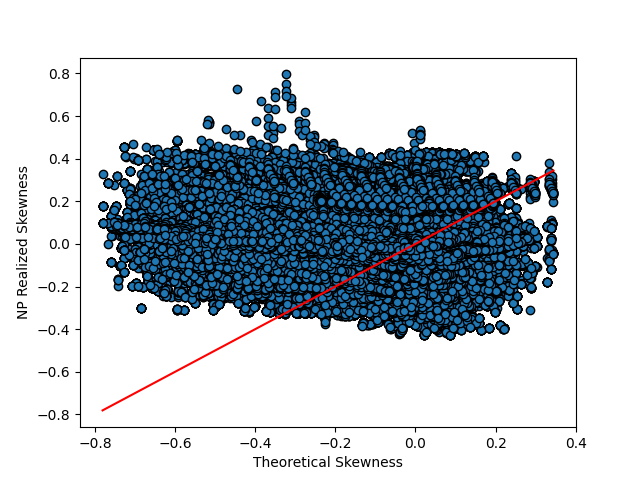
\includegraphics[width=\textwidth]{img/theoretical_skewness_vs_NP_rskewness_feller_condition_true.png}
        \caption{Theoretical Skewness vs Skewness from Neuberger \& Payne (2021)}
    \end{subfigure}
    \bigskip % https://tex.stackexchange.com/questions/475149/using-subfigure-and-creating-two-rows-of-figures
    \begin{subfigure}[b]{0.4\textwidth}
        \centering
        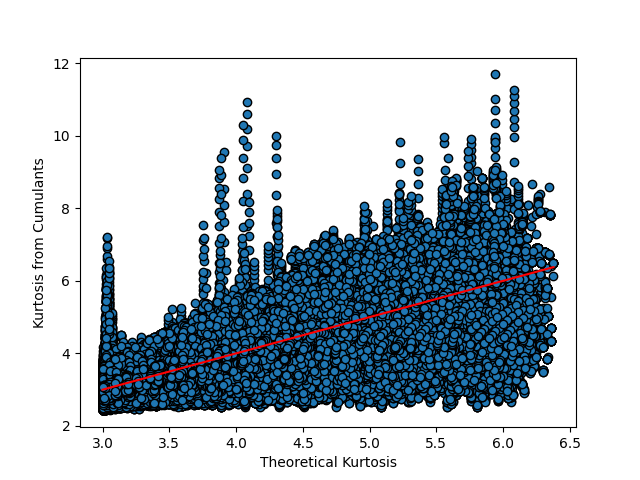
\includegraphics[width=\textwidth]{img/theoretical_kurtosis_vs_kurtosis_from_cumulants_feller_condition_true.png}
        \caption{Theoretical Kurtosis vs Kurtosis from Cumulants}
    \end{subfigure}
    \hfill
    \begin{subfigure}[b]{0.4\textwidth}
        \centering
        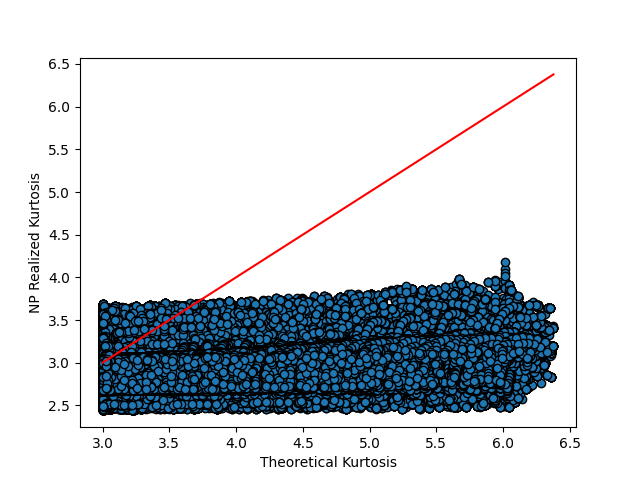
\includegraphics[width=\textwidth]{img/theoretical_kurtosis_vs_NP_rexcess_kurtosis_feller_condition_true.png}
        \caption{Theoretical Kurtosis vs Kurtosis from Neuberger \& Payne (2021)}
    \end{subfigure}
    \caption{Comparison of the theoretical skewness and kurtosis with the skewness and kurtosis from the Cumulants and the real skewness and kurtosis from Neuberger \& Payne (2021) for simulations where the Feller condition is fulfilled. Invalid simulations are excluded.}
    \label{fig:theoretical_vs_real_skewness_kurtosis}
\end{figure}

- Wir untersuchen nun, ob es Zusammenhänge zwischen den Parametern des Heston-Modells und den p Werten des Kolmogorov-Smirnov-Tests gibt. Abbildung \ref{fig:pairplot_GC_cum_KS_muzero} zeigt einen Pairplot für alle Parameterkombinationen (außer $\mu$) und die p Werte des Kolmogorov-Smirnov-Tests für die Gram-Charlier Expansion
mit Kumulanten gegen die theoretische Dichte. Je heller die Region ist, desto höher ist der Anteil an p values über 5\% und damit desto öfter approximiert die Gram-Charlier Expansion mit Kumulanten die theoretische Dichte gut.
- Man sieht in den Farbverläufen, welche Parameter einen Einfluss zu haben scheinen, das trifft auf $\sigma$, $\kappa$ und $\theta$ zu. Der Parameter $\rho$ scheint eher keinen Einfluss haben, egal wie man diesen Parameter wählt und den anderen Parameter fixiert, die Farbe ändert sich nicht. Selbiges gilt für $v_0$. Man würde auch erwarten, dass $v_0$ keinen Einfluss hat, da $v_0$ die Startvolatilität ist und wir, um die unbedingten Momente und Kumulanten zu bestimmen, einen Burnin von 3 Jahren (bei 15 Jahren Simulationsdauer) verwenden. 
- Für den Parameter $\sigma$ sieht man, dass dieser so gering wie möglich sein sollte, während $\kappa$ so hoch wie möglich sein sollte. Die Wahl des Parameters $\theta$ scheint schwieriger zu sein, da es keine klare Tendenz gibt. Grundsätzlich scheint $\theta$ mit steigendem $\kappa$ auch größer gewählt werden, zum anderen sollte bei kleinem $\sigma$ auch ein kleines $\theta$ gewählt werden. Eine Darstellung aller 3 Parameter in einem 3D-Plot zeigt Abbildung \ref{fig:GC_cum_KS_3d_p_value_sigma_kappa_theta_muzero}.

\begin{figure}
    \centering
    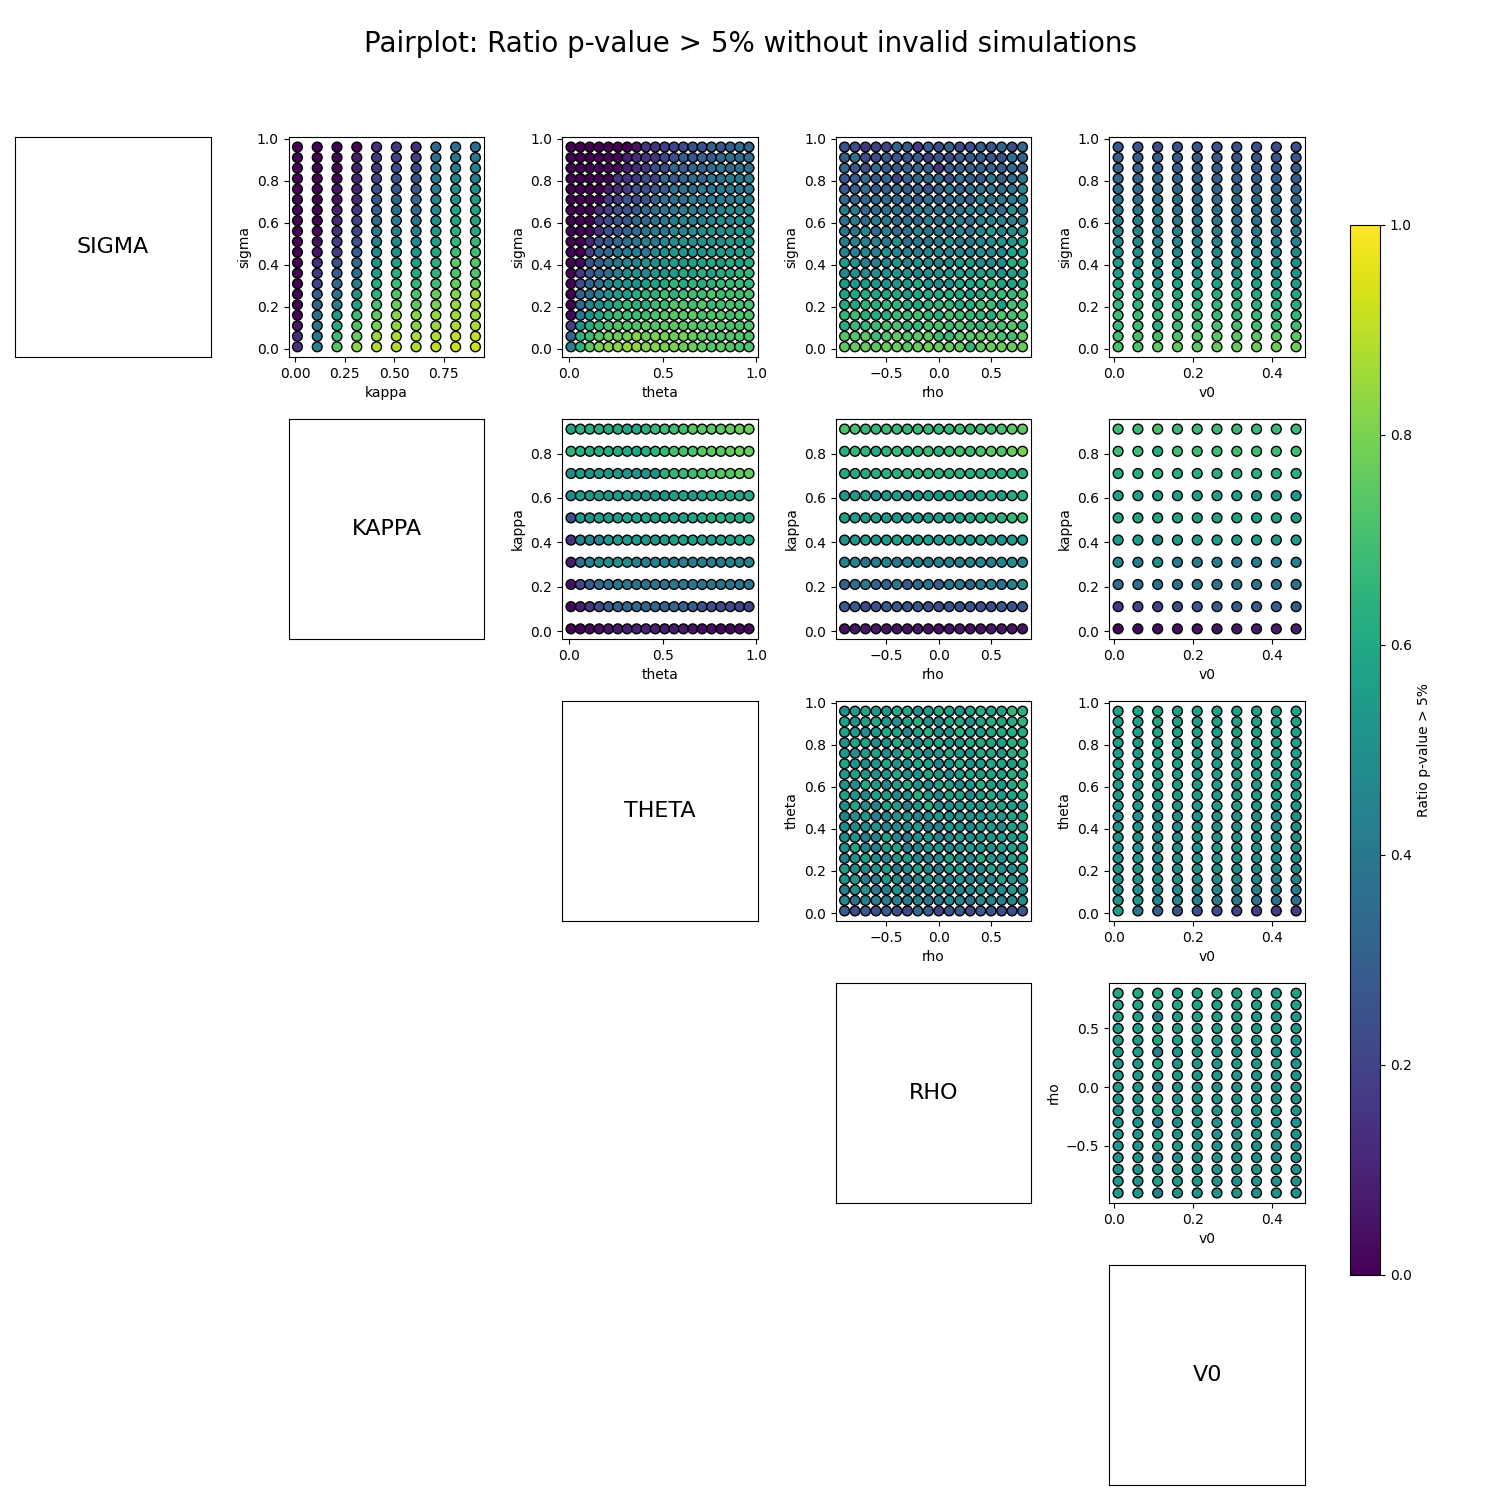
\includegraphics[width=0.8\textwidth]{img/pairplot_GC_cum_KS_muzero.png}
    \caption{Pairplot for each pair of parameters for the Heston Model and the percentage of p values of the Kolmogorov-Smirnov-Test for the Gram-Charlier Expansion with Cumulants vs the theoretical density above 5\%. Invalid simulations are excluded and $\mu=0$.}
    \label{fig:pairplot_GC_cum_KS_muzero}
\end{figure}

\begin{figure}
    \centering
    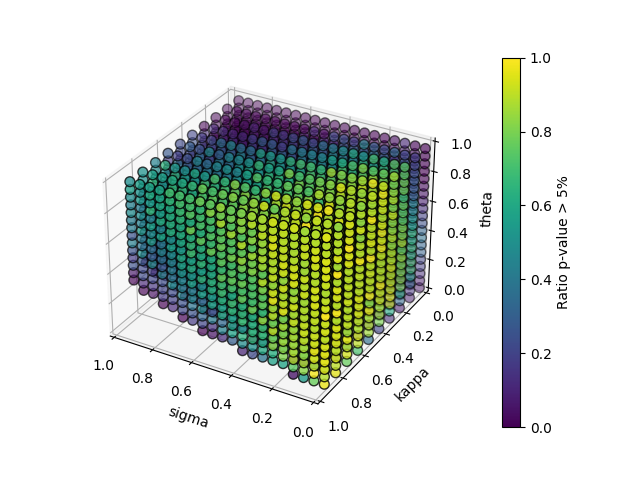
\includegraphics[width=0.8\textwidth]{img/GC_cum_KS_3d_p_value_sigma_kappa_theta_muzero.png}
    \caption{Percentage of simulations where the p-value of the Kolmogorov-Smirnov-Test against the theoretical density is above 5\%. Invalid simulations are excluded. $\mu=0$}
    \label{fig:GC_cum_KS_3d_p_value_sigma_kappa_theta_muzero}
\end{figure}

- Es ist sehr schwer, allgemeingültige Aussagen, welche Parameterkombinationen zu guten Ergebnissen führen, zu treffen. insbesondere grafische Visualisierungen haben das Problem, dass man nicht ausreichend Dimensionen darstellen kann. Daher Einsatz von Klassifizierungsmethoden, die nicht auf grafischer Darstellung basieren, wie z.B. die logistische Regression und Random Forest. Dazu wurden alle gültigen Simulationen genommen und in 80\% Trainings- und 20\% Testdaten aufgeteilt. Die unabhängigen Variablen $X$ sind die Parameter des Heston-Modells, die abhängige Variable $y$ ob der p-value des KS-tests größer als 5\% ist. Die Gruppen sind nicht gleich groß, 60.98\% der Simulationen haben einen p-value über 5\%. Die logistische Regression hat eine Accuracy von 79.53\%, der Random Forest, bestehend aus 100 Decision Trees, eine Accuracy von 91.59\%. Die Precision für $y=1$ beträgt 82\% bzw. 92\%. Die Precision ist relevant, weil sie den Anteil der True Positives an allen Positives angibt und ein geringer Wert hier bedeuten würde, dass Parameterkombinationen, die keine Approximation mittels Gram-Charlier zulassen würden, mit Gram-Charlier approximiert werden. Wenn auf dieser Basis Preise für Wertpapiere gefunden werden sollen, so könnte dies zu großen Verlusten führen.
- Schaut man sich die Koeffizienten der logistischen Regression (siehe Tabelle \ref{tab:logistic_regression_coefficients}) oder den Feature Importance des Random Forests (siehe Abbildung \ref{fig:feature_importances}) an, so stellt man fest, dass $\sigma$ mit Abstand der wichtigste Parameter ist. $\theta$ und $\kappa$ sind auch wichtig, aber welcher von beiden wichtiger ist, darüber sind sich die Modelle nicht einig. Auch welche Rolle $\rho$ spielt, ist nicht klar: In der logisitischen Regression nicht, im Random Forest schon. $\mu$ und $v_0$ spielen keine Rolle. Alle Parameter sind auch statistisch signifikant.

\begin{table}
    \centering
    \begin{tabular}{l|c}
        \textbf{Parameter} & \textbf{Coefficient} & \textbf{Standard Error} & $z$ & $\mathbb{P}>\vert z\vert$ \\
        \hline
        const & -0.8708 & 0.010 & -84.332 & 0.000 \\
        $\mu$ & -1.2841 & 0.111 & -11.568 & 0.000 \\
        $\sigma$ & -7.2015 & 0.017 & -429.506 & 0.000 \\
        $\kappa$ & 4.4584 & 0.014 & 318.689 & 0.000 \\
        $\theta$ & 3.0120 & 0.013 & 237.146 & 0.000 \\
        $\rho$ & 0.4219 & 0.005 & 78.359 & 0.000 \\
        $v_0$ & -0.0728 & 0.019 & -3.765 & 0.000
    \end{tabular}
    \caption{Coefficients of the logistic regression}
    \label{tab:logistic_regression_coefficients}
\end{table}

\begin{figure}
    \centering
    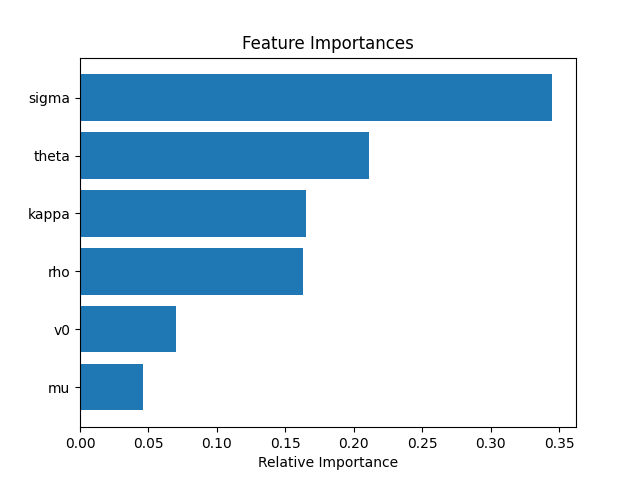
\includegraphics[width=0.8\textwidth]{img/feature_importances.png}
    \caption{Feature Importances of the Random Forest}
    \label{fig:feature_importances}
\end{figure}

\section{Comparing the Expansion Methods}

\subsection{General Approximation}
- Bisher haben wir die Ergebnisse Gram-Charlier-Expansion aus vielen Perspektiven betrachtet, aber es stellt sich die Frage, ob sich Expansionsmethoden überhaupt lohnen? Dazu vergleichen wir in einem ersten Schritt, ob das hinzufügen des 3. und 4. Kumulanten die Ergebnisse verbessert, und zwar in Abhängigkeit der theoretischen Skewness und Kurtosis. Als Expansionsmethode, die nur die ersten beiden Kumulanten verwendet, wählen wir die Normalverteilung wobei die Kumulanten die Parameter $\mu$ und $\sigma$ bestimmen (see \ref{fig:gc_vs_no_theoretical_skewness_kurtosis}).
- Man sieht, dass es sich lohnt, eine komplexere Expansionsmethode als die Normalverteilung zu nutzen, da sich die Ergebnisse für gegebene Skewness und Kurtosis verbessern.

\begin{figure}
    \centering
    \begin{subfigure}[b]{0.4\textwidth}
        \centering
        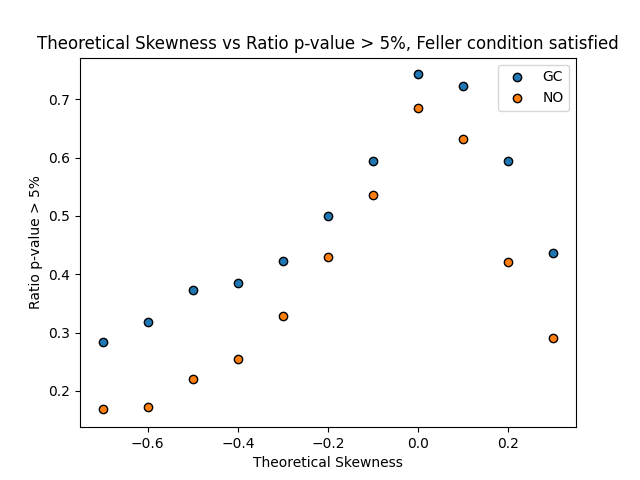
\includegraphics[width=\textwidth]{img/theoretical_skewness_vs_ratio_feller_condition_true.png}
        \caption{Theretical Skewness}
    \end{subfigure}
    \hfill
    \begin{subfigure}[b]{0.4\textwidth}
        \centering
        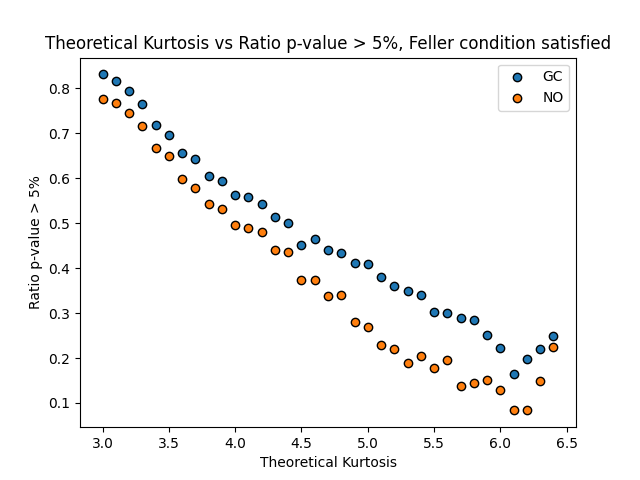
\includegraphics[width=\textwidth]{img/theoretical_kurtosis_vs_ratio_feller_condition_true.png}
        \caption{Theoretical Kurtosis}
    \end{subfigure}
    \caption{Ratio of simulations where the p-value of the Kolmogorov-Smirnov-Test against the theoretical density is above 5\% in relation to the theoretical skewness and kurtosis. GC stands for the Gram-Charlier-Expansion while NO stands for the Normal Distribution. Feller condition is fulfilled.}
    \label{fig:gc_vs_no_theoretical_skewness_kurtosis}
\end{figure}

\begin{figure}
    \centering
    \begin{subfigure}[b]{0.4\textwidth}
        \centering
        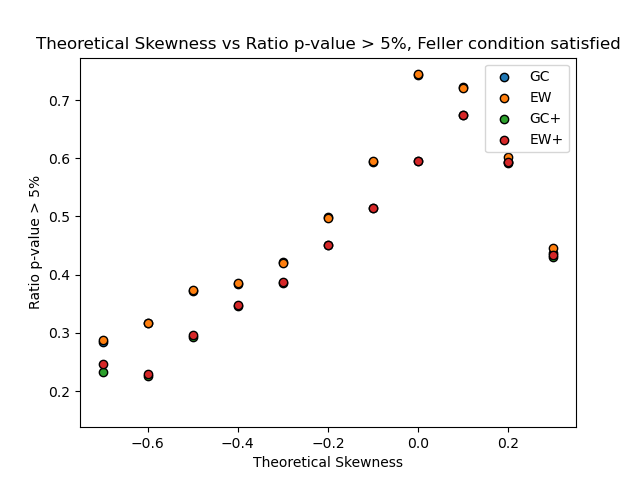
\includegraphics[width=\textwidth]{img/theoretical_skewness_vs_ratio_gc_ew_feller_condition_true.png}
        \caption{Theretical Skewness}
    \end{subfigure}
    \hfill
    \begin{subfigure}[b]{0.4\textwidth}
        \centering
        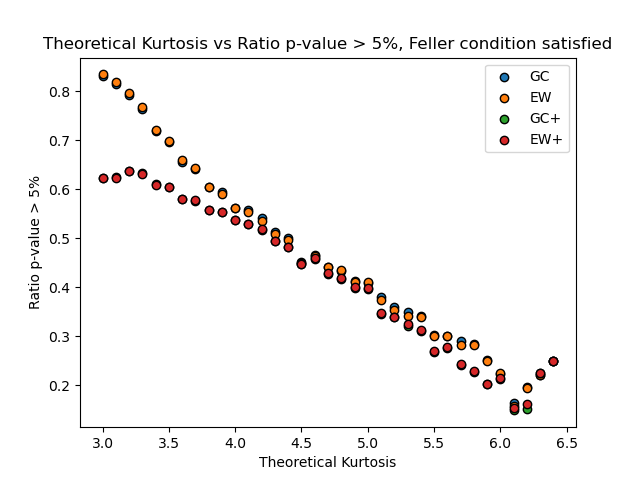
\includegraphics[width=\textwidth]{img/theoretical_kurtosis_vs_ratio_gc_ew_feller_condition_true.png}
        \caption{Theoretical Kurtosis}
    \end{subfigure}
    \caption{Ratio of simulations where the p-value of the Kolmogorov-Smirnov-Test against the theoretical density is above 5\% in relation to the theoretical skewness and kurtosis. GC stands for the Gram-Charlier-Expansion, EW for the Edgeworth-Expansion. A + behind the Expansion denotes the variant with positivity constraints. Feller condition is fulfilled.}
    \label{fig:gc_vs_ew_theoretical_skewness_kurtosis}
\end{figure}

- Ein ähnliches Bild ergibt sich im Vergleich der Gram-Charlier-Expansion und Edgeworth-Expansion mit ihren Varianten, die durch die Positivitätsbedingung eingeschränkt sind. Die Ergebnisse sind in Abbildung \ref{fig:gc_vs_ew_theoretical_skewness_kurtosis} dargestellt und man erkennt, dass die positivitätsbeschränkten Varianten deutlich schlechter abschneiden. Das liegt an dem Verzerrungseffekt, den die Positivitätsbedingung mit sich bringt. Es kann auch keine Abhängigkeit von einzelnen Parametern des Heston-Modells festgestellt werden, bei der die positivitätsbeschränkten Varianten besser abschneiden. Allerdings führen die gewählten Parameterkombinationen für die Simulation auch nie zu theoretischen Skewness- oder Kurtosis-Werten, die außerhalb des Gültigkeitsbereichs der Expansionsmethoden liegen, sodass diese negative Werte, und damit keine Dichte mehr, liefern würden.

- In der Datenbank kann man nach Parameterkombinationen suchen, bei denen sich die Edgeworth-Expansion lohnt, das heißt der p value für den Kolmogorov-Smirnov-Test ist für die Edgeworth-Expansion größer als bei der Gram-Charlier-Expansion und liegt über 5\%, während zeitgleich der p value für die Gram-Charlier-Expansion unter 5\% liegt. Insgesamt werden 2866 solcher Parameterkombinationen gefunden, aus insgesamt 501713 möglichen (wie üblich wurden ungültige Simulationen entfernt). Das entspricht einem Anteil von 0.57\%.

\subsection{Approximation of the Tails}
- Um die Tails zu vergleichen nutzen wir den Anderson-Darling-Test. Ein Verleich mittels des Hill-Estimators zur Schätzung des Tail-Index wurde ebenfalls versucht, es war aber nicht möglich ein Plateau im Hill-Plot zu erkennen, was darauf hindeutet, dass die Tails nicht fat genug sind, wie z.B. in der Pareto-Verteilung. Das ist aber ein essentielles Kriterium, um den Hill-Estimator anwenden zu können. 

- Man könnte vermuten, dass sich die Ergebnisse ändern, wenn man nun einen Test verwendet, der stärker auf die Ränder der Verteilung reagiert, wie den Anderson-Darling-Test. Aber man sieht, dass es praktisch keinen Unterschied zwischen den Abbildungen \ref{fig:pairplot_GC_cum_AD_muzero} + \ref{fig:pairplot_GC_cum_AD_mu005} und den Abbildungen \ref{fig:pairplot_GC_cum_KS_muzero} + \ref{fig:pairplot_GC_cum_KS_mu005} gibt. Das lässt den Schluss zu, dass die Gram-Charlier-Expansion auf Basis von Cumulants auch die Tails gut approximieren kann.

\begin{figure}
    \centering
    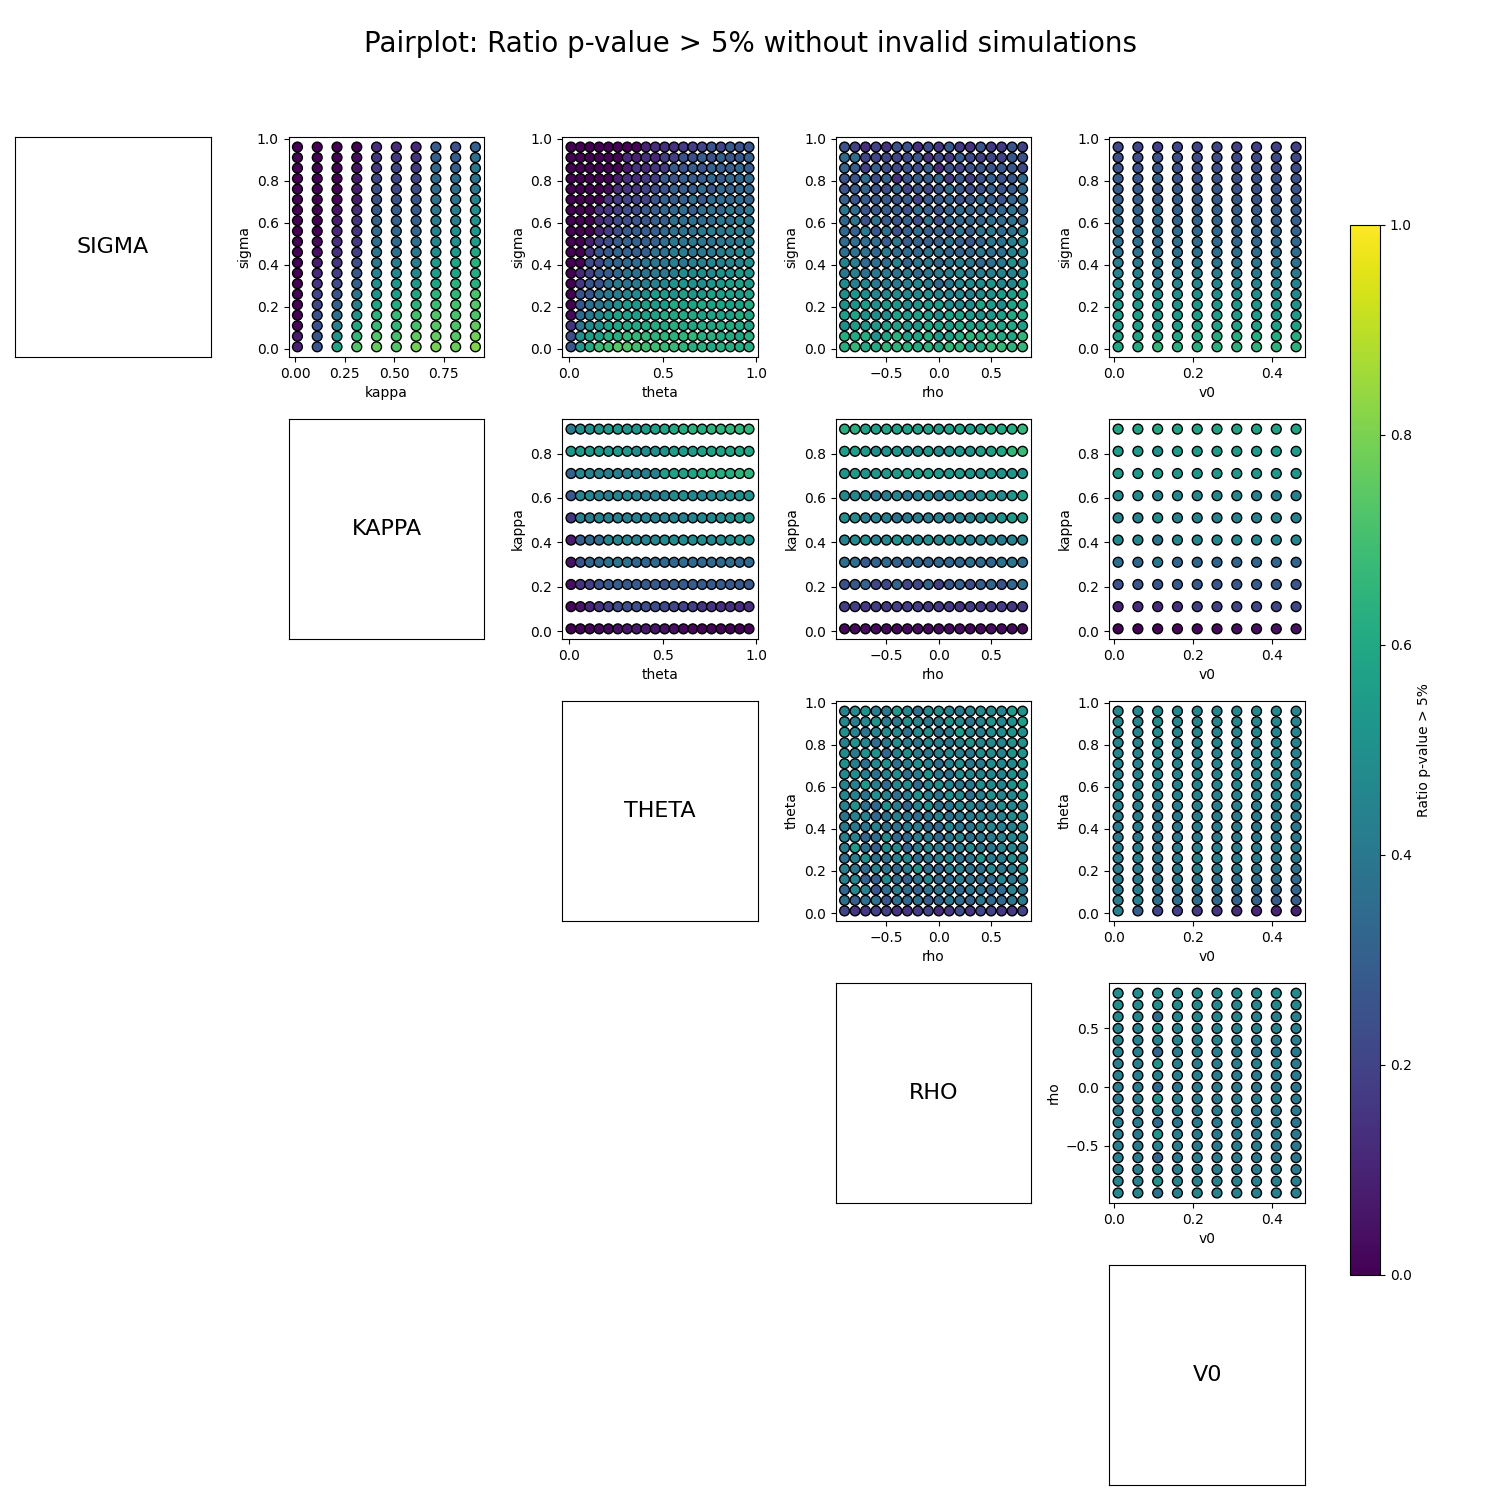
\includegraphics[width=0.8\textwidth]{img/pairplot_GC_cum_AD_muzero.png}
    \caption{Pairplot for each pair of parameters for the Heston Model and the percentage of p values of the Anderson-Darling-Test for the Gram-Charlier Expansion with Cumulants vs the theoretical density above 5\%. Invalid simulations are excluded and $\mu=0$.}
    \label{fig:pairplot_GC_cum_AD_muzero}
\end{figure}

\begin{figure}
    \centering
    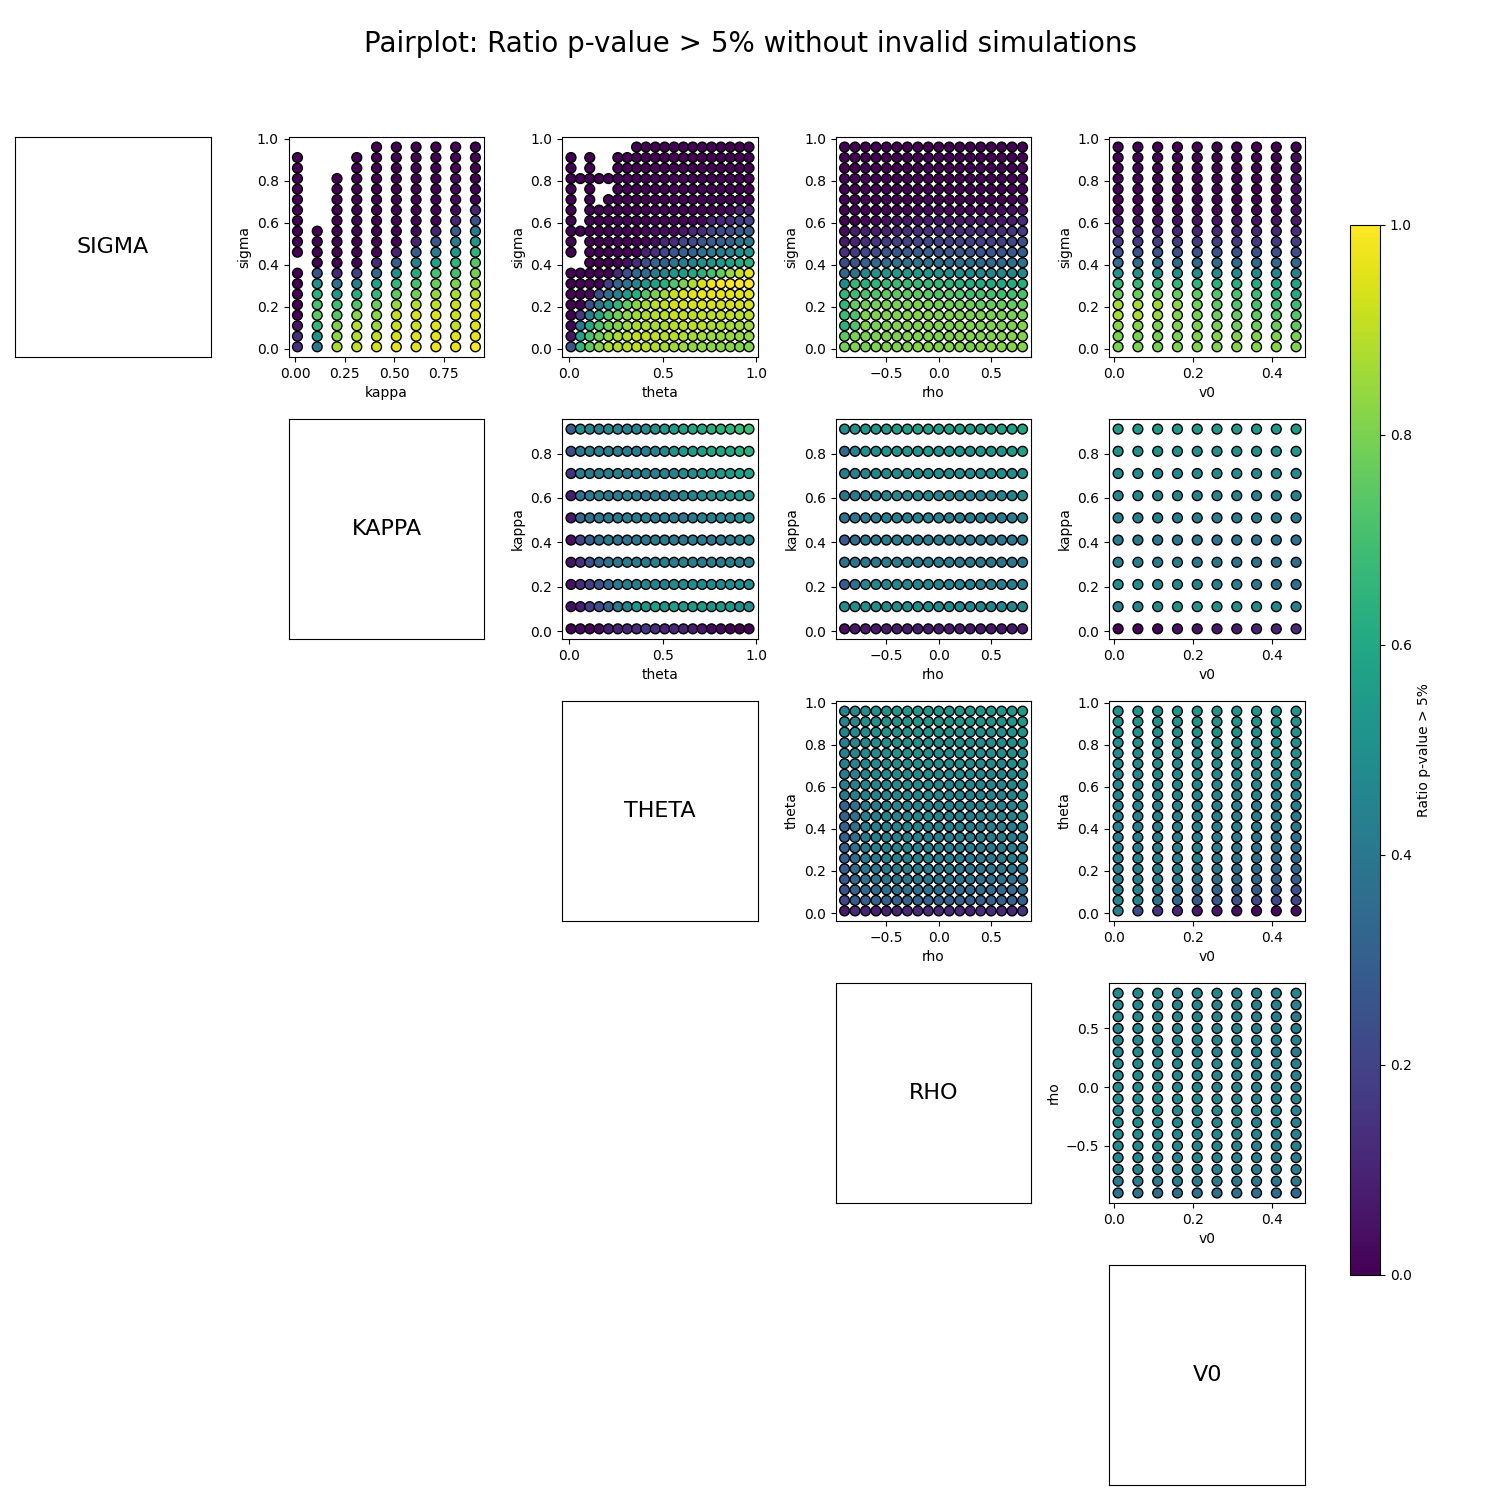
\includegraphics[width=0.8\textwidth]{img/pairplot_GC_cum_AD.png}
    \caption{Pairplot for each pair of parameters for the Heston Model and the percentage of p values of the Anderson-Darling-Test for the Gram-Charlier Expansion with Cumulants vs the theoretical density above 5\%. Invalid simulations are excluded and $\mu=0.05$.}
    \label{fig:pairplot_GC_cum_AD_mu005}
\end{figure}